\subsection{Design and interface}
\subsubsection{Transmitter}

The transmitter takes an asynchronous data signal as input. The driver stage then inverts and amplifies the signal which then drives the LED. If the signal is high then the LED is turned off and if the signal is low then the LED is turned on.

\begin{figure}[h]
\centering
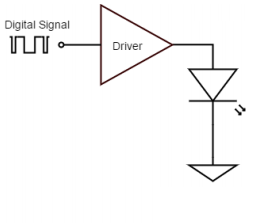
\includegraphics[width=0.4\textwidth]{trans}
\caption{The transmitter}
\label{fig:trans}
\end{figure}

\subsubsection{Receiver}
The flashing pulses from the LED excites the photodiode and converts the light into current. The current is then converted to a voltage and passed through an amplifier. Since the signal to noise ratio is very low both ambient noise and fluorescent light needs to be filtered out from the signal which is accomplished by the high pass filter. Finally the signal gets reconstructed through a schmitt trigger.

\begin{figure}[h]
\centering
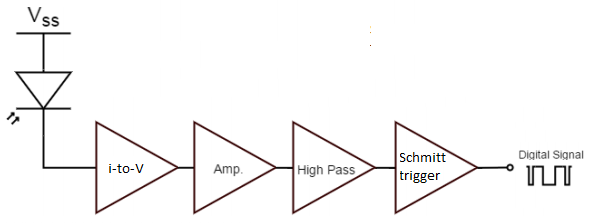
\includegraphics[width=0.8\textwidth]{rec}
\caption{The receiver}
\label{fig:rec}
\end{figure}